\section{Desarrollo}

\subsection{Rerequerimientos}

Para este trabajo practico se nos solicita realizar un circuito resonante que cumpla con las siguientes especificaciones:

\begin{itemize}
    \item Frecuencia de resonancia: $f_0 = 16 MHz$
    \item Ancho de banda: $BW = 1.6 MHz$
    \item Factor de calidad con el circuito cargado: $Q_c = 10$
    \item Impedancia de entrada: $Z_{in} = 50 \Omega$
    \item Impedancia de salida: $Z_{out} = 1 k\Omega$
\end{itemize}

\subsection{Diseño}

El primer paso para construir el circuito resontate es realizar los calculos del inductor. Para ello, se utilizara la siguiente formula:

% L = D^3 * Ns^2 k 10^-3 [micro H]
\begin{equation}
    L = D^3 \cdot N_s^2 \cdot k \cdot 10^{-3} [\mu H]
\end{equation}

Donde $D$ es el diametro externo del inductor, $N_s$ es el numero de espiras por unidad de longitud y $k$ es la constante de Nagaoka. 
Para comenzar fijaremos valores que nos permitan ajustar a los calculos. Por lo tanto, se fija:

\begin{itemize}
    \item $D =  2.21 cm$
    \item diametro del conductor: $d = 2.1\; \text{mm}$
    \item separacion entre espiras: : $S = 3\; \text{mm}$
\end{itemize}

Con estos valores, se puede calcular el numero de espiras por unidad de longitud:

\begin{equation}
    N_s = \frac{1}{S + d} = \frac{10}{3 + 2.1 } = 2\; \text{espiras/cm}
\end{equation}

Para seguir con los calculos necesitaremos seleccionar un valor de longitud del inductor $L$. En la planilla de calculo se definieron valores de longitud con un paso de 0.1 cm.
Finalmente seleccionamos:

% separar unidad de numero 
\begin{itemize}
    \item $L = 3.8\; \text{cm}$
\end{itemize}

Calculamos la cantidad de espiras:

\begin{equation}
    N = N_s \cdot L = 2 \cdot 3.8 = 7\; \text{espiras} 
\end{equation}

Tenemos que tener en cuenta que redondeamos para Ns de 1.96 a 2. Ahora calculamos la relacion de longitud con diametro:

\begin{equation}
    \frac{L}{D} = \frac{3.8}{2.21} = 1.72
\end{equation}

Ahora tendremos que calcular la constante de Nagaoka, para esto hay dos formas de hacerlo. La primera es mediante la siguiente formula:

% k = K * Pi ^2 * L/D
\begin{equation}
    k = K \cdot \pi^2 \cdot \frac{L}{D} 
\end{equation}

Donde $K$ se calcula mediante la siguiente formula:

% K = 1 / (1 + 0.9 D/2L - 2*10^-2 (D/2L)^2)
\begin{equation}
    K = \frac{1}{1 + 0.9 \cdot \frac{D}{2L} - 2 \cdot 10^{-2} \left(\frac{D}{2L}\right)^2}
\end{equation}

Sustituyendo los valores obtenemos:

\begin{equation}
    K = \frac{1}{1 + 0.9 \cdot \frac{2.21}{2 \cdot 3.8} - 0.2 \cdot 10^{-2} \left(\frac{2.21}{2 \cdot 3.8}\right)^2} = 0.79
\end{equation}

Y el factor de Nagaoka:

\begin{equation}
    k = 0.79 \cdot \pi^2 \cdot 1.72 = 13.5
\end{equation}

La otra forma es graficamente, donde con L/D = 1.72 ingresamos al siguiente grafico:

\begin{figure}[h]
    \centering
    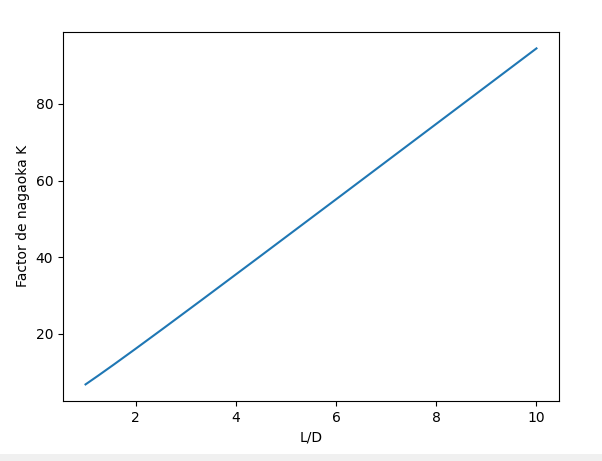
\includegraphics[width=0.5\textwidth]{Imagenes/factorNagaoka.png}
    \caption{Curva de Nagaoka K}
\end{figure}

Con todos estos parametros calculadores, podemos calcular el valor de la inductancia:

\begin{equation}
    L = D^3 \cdot N_s^2 \cdot k \cdot 10^{-3} = 2.21^3 \cdot 2^2 \cdot 13.5 \cdot 10^{-3} = 0.56\; \mu H
\end{equation}

\subsubsection{Calculo de resistencias}

Para el calculo de las resistencias necesitaremos calcular el factor de calidad sin carga $Q_d$, con la siguiente formula:

\begin{equation}
    Q_d = 8850 \cdot \frac{D \cdot L}{102 \cdot L + 45 \cdot D} \cdot \sqrt{f_0}
\end{equation}

Donde $L$ es la longitud del inductor en cm, $D$ es el diametro del inductor en cm y $f_0$ es la frecuencia de resonancia en MHz. Sustituyendo los valores obtenemos:

\begin{equation}
    Q_d = 610.4 
\end{equation}

La reactancia del inductor es:

\begin{equation}
    X_L = 2 \cdot \pi \cdot f_0 \cdot L = 2 \cdot \pi \cdot 16 \cdot 10^6 \cdot 0.56 \cdot 10^{-6} = 56\; \Omega
\end{equation}

Con $X_L$ y $Q_d$ podemos calcular la resistencia paralela $R_p$:

\begin{equation}
    R_p = Q_d \cdot X_L = 610.4 \cdot 56 = 34300\; \Omega
\end{equation}

Con $Q_C$ y $X_L$ podemos calcular la resistencia total $R_t$:

\begin{equation}
    R_t = \frac{X_L}{Q_c} = \frac{56}{10} = 560\; \Omega
\end{equation}

Con los valores calculados podremos calcular la resistencia de carga reflejada $R_L'$ y la resistencia del generador reflejada $R_g'$, para esto tenemos que despejar $R_L'$ y $R_g'$ de la ecuacion 8:

\begin{equation}
    R_L' // R_P = 2 \cdot R_T 
\end{equation}

\begin{equation}
    R_g' = 2 \cdot R_T 
\end{equation}

Despejando $R_L'$ obtenemos:

\begin{equation}
    R_L' = \frac{2 \cdot R_T \cdot R_P}{R_P - 2 \cdot R_T} 
\end{equation}

Sustituyendo los valores obtenemos:

\begin{equation}
    R_L' = \frac{2 \cdot 560 \cdot 34300}{34300 - 2 \cdot 560} = 1161.8\; \Omega
\end{equation}

Y calculando $R_G'$:

\begin{equation}
    R_g' = 2 \cdot 560 = 1123\; \Omega
\end{equation}


% subsection de la subsection de diseño
\subsubsection{Calculo del capacitor}

Con la frecuencia de resonancia $f_0 = 16 MHz$ y el valor de la inductancia calculado, podemos calcular el valor del capacitor:

\begin{equation}
    C = \frac{1}{L \cdot (2 \cdot \pi \cdot f_0)^2} = \frac{1}{0.56 \cdot (2 \cdot \pi \cdot 16 \cdot 10^6)^2} = 177\; \text{pF}
\end{equation}

Con las ecuaciones de la formula 13, podemos calcular $C_1$, $C_2$, $C_3$ y $C_4$:

\begin{equation}
    C_2 = \frac{C}{2} \cdot \sqrt{\frac{R_g'}{R_g}}
\end{equation}

Entonces $C_1$ sera igual a: 

\begin{equation}
    C_1 = \frac{C_2}{\sqrt{R_g' / R_g - 1}}
\end{equation}

Con $C_4$ y $C_3$ nos queda:

\begin{equation}
    C_4 = \frac{C}{2} \cdot \sqrt{\frac{R_L'}{R_L}}
\end{equation}

\begin{equation}
    C_3 = \frac{C_4}{\sqrt{R_L' / R_L - 1}}
\end{equation}

Remplazando los valores obtenemos:


\begin{equation}
    C_1 = 112\; \text{pF}
\end{equation}

\begin{equation}
    C_2 = 420\; \text{pF}
\end{equation}

\begin{equation}
    C_3 = 1225\; \text{pF}
\end{equation}

\begin{equation}
    C_4 = 95\; \text{pF}
\end{equation}

\newpage
\subsection{Simulacion}

Para comprobar el correcto funcionamiento de nuestro circuito, se realizo una simulacion en LTSpice. A continuacion se muestra el circuito simulado:

\begin{figure}[h]
    \centering
    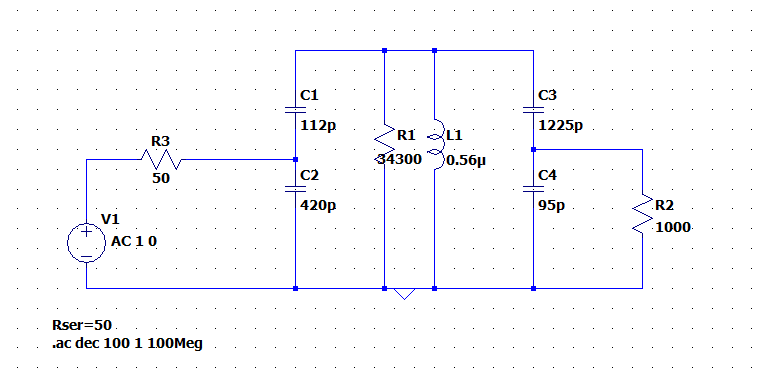
\includegraphics[width=0.7\textwidth]{Imagenes/circuito.png}
    \caption{Circuito simulado en LTSpice}
\end{figure}

El resultado de la simulacion es el siguiente:

\begin{figure}[h]
    \centering
    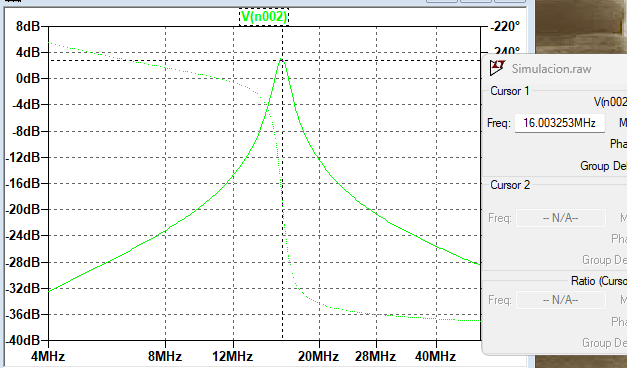
\includegraphics[width=0.7\textwidth]{Imagenes/resultado_circuito.png}
    \caption{Respuesta en frecuencia del circuito simulado}
\end{figure}

Se observa que la frecuencia de resonancia es de $16 MHz$ con una ganancia de $2 dB$. Ademas:

\begin{itemize}
    \item frecuencia de corte inferior: $15.2 MHz$
    \item frecuencia de corte superior: $16.8 MHz$
    \item ancho de banda: $1.6 MHz$
    \item $Q_c = 10$
\end{itemize}

\newpage
\subsection{Seleccion de componentes y armado}

El primer paso sera determinar que capacitores utilizaremos para el circuito. Los capacitores seleccionados son:

\begin{itemize}
    \item $C_1 = 100\; \text{pF}$
    \item $C_2 = 330 + 100 = 430\; \text{pF}$
    \item $C_3 = 1000 + 100 + 100 =1200\; \text{pF}$
    \item $C_4 = 100\; \text{pF}$
\end{itemize}

La capacidad total sera:

\begin{equation}
    C_T = \frac{C_1 \cdot C_2}{C_1 + C_2} + \frac{C_3 \cdot C_4}{C_3 + C_4} 
\end{equation}

\begin{equation}
    C_T = 173.4 \; \text{pF}
\end{equation}

El resultado obtenido con los capacitores obtenidos, haciendo un analisis de montecarlo:

\begin{figure}[h]
    \centering
    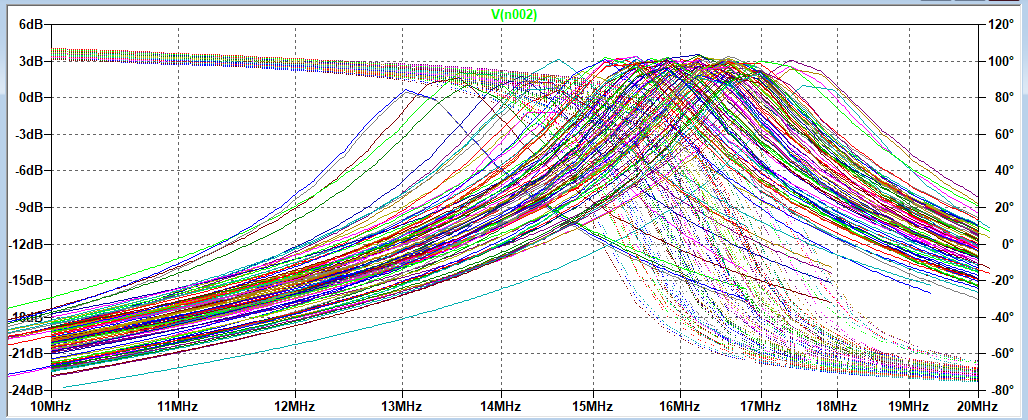
\includegraphics[width=0.7\textwidth]{Imagenes/montecarlo.png}
    \caption{Analisis de montecarlo}
\end{figure}

Vemos que la tolerancia y los capacitores utilizados hace que $f_0$ varie entre $13 MHz y 17.2 MHz$.


El inductor y los capacitores montados en la PCB finalmente nos queda:

\begin{figure}[h]
    \centering
    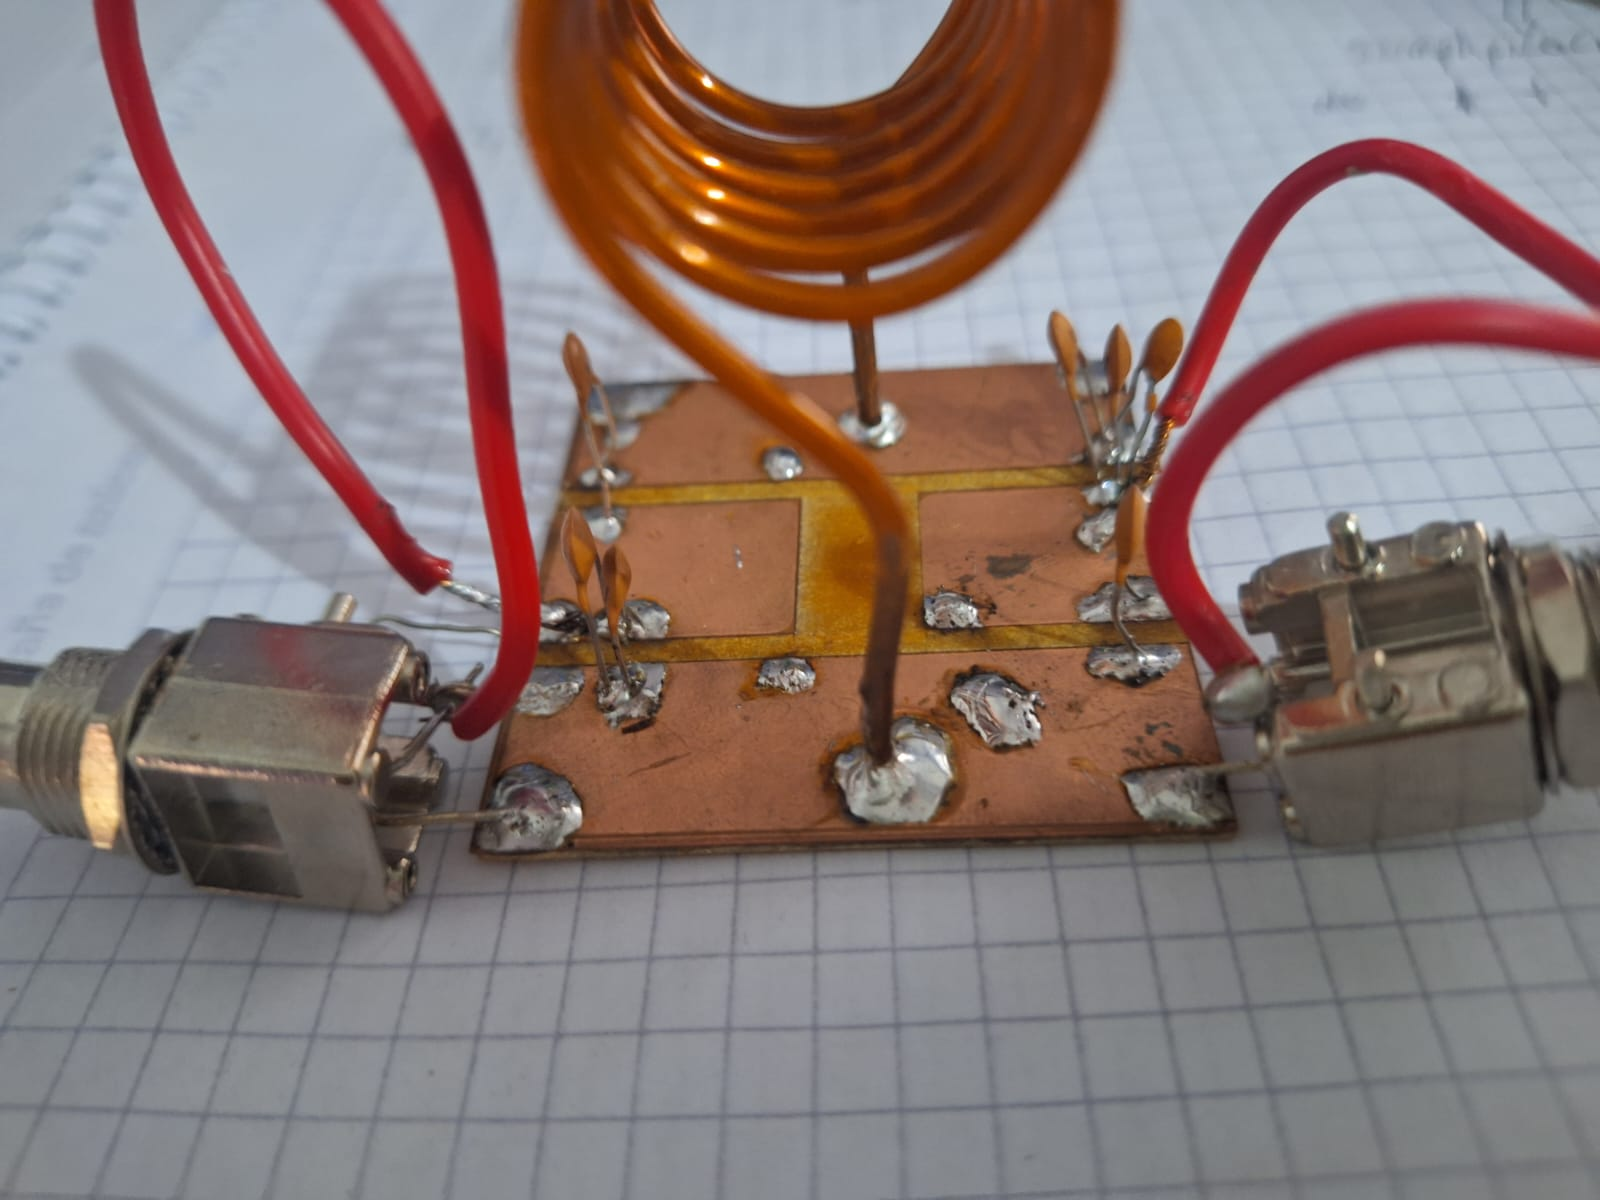
\includegraphics[width=0.7\textwidth]{Imagenes/pcb1.jpeg}
    \caption{PCB montada}
\end{figure}

\begin{figure}[h]
    \centering
    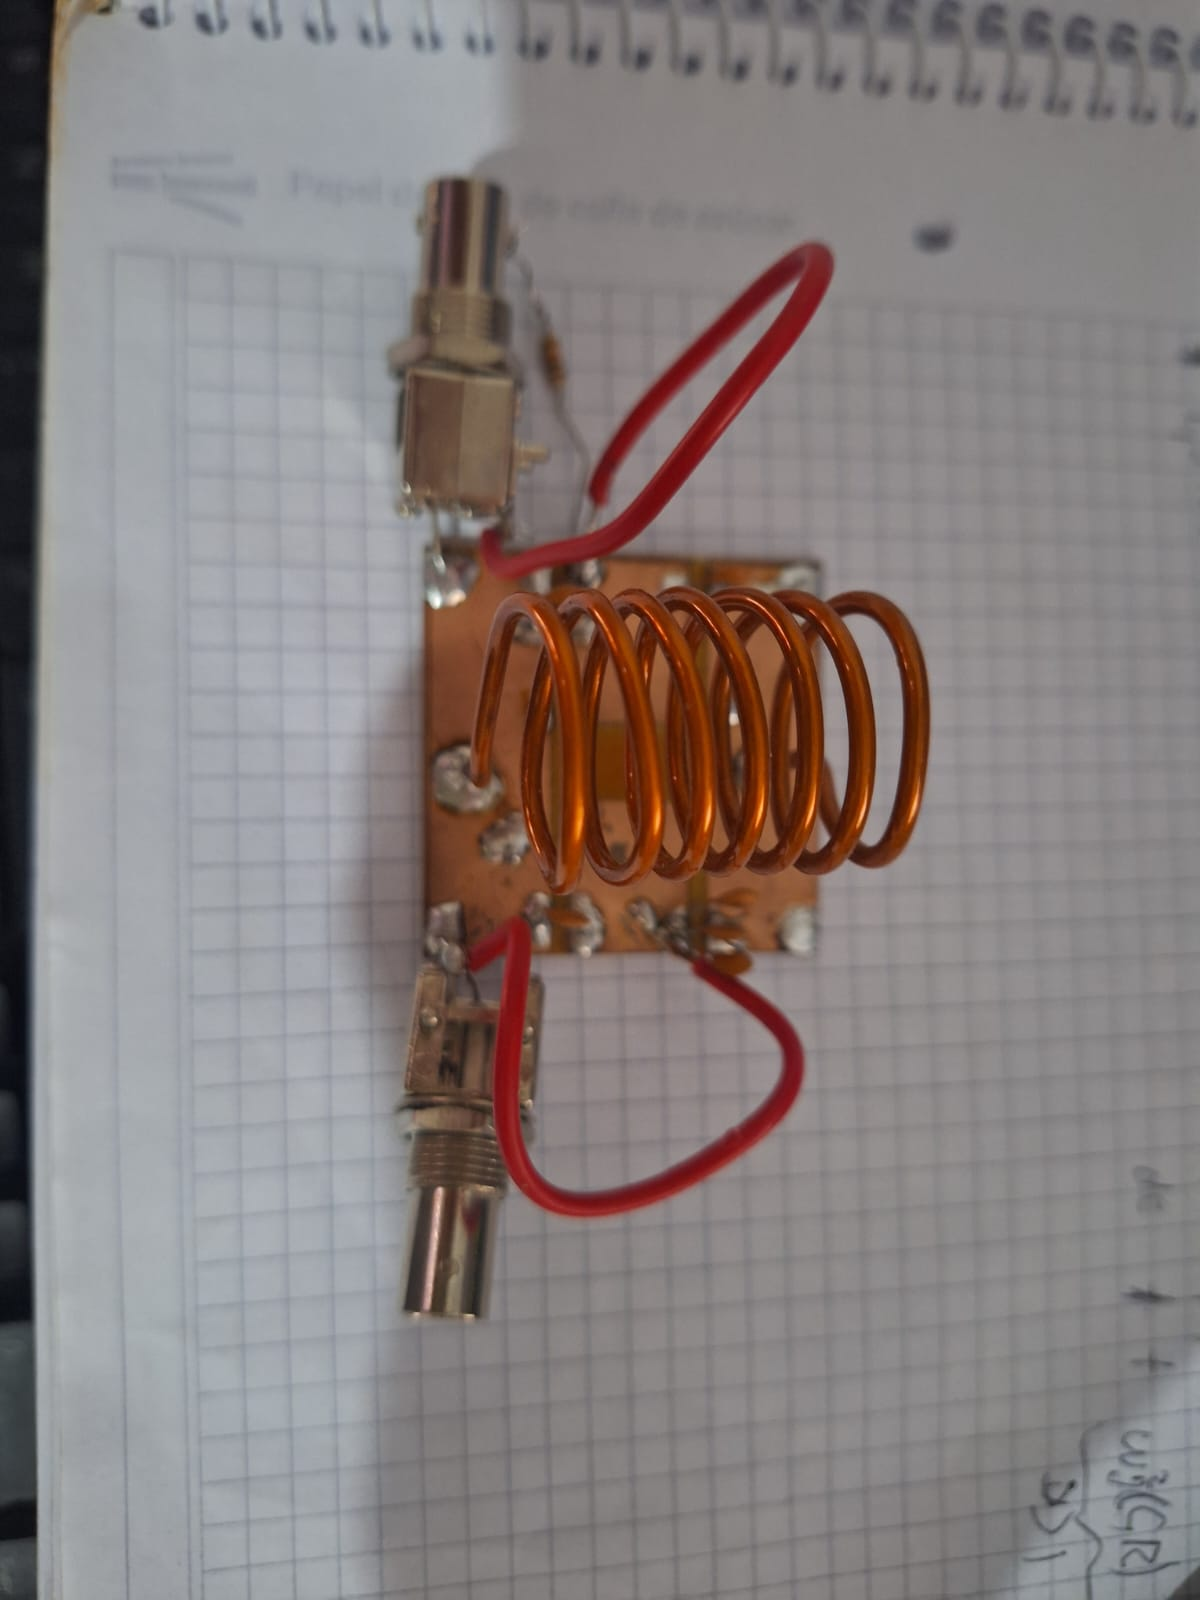
\includegraphics[width=0.7\textwidth]{Imagenes/pcb2.jpeg}
    \caption{PCB montada}
\end{figure}

